\section{Photovoltaic generation}

The generation of direct current electricity from solar energy is a phenomenom known as \textit{Photovoltaic effect} which was first discovered by a French physicist named Edmond Becquerel in 1839 \cite{PVeffect}. This process allows the generation of electrical energy in a solar cell, which is composed of two layers of semiconductor material (usually silicon), when it is exposed to the sunlight \cite{PVeffect}. The greater the intensity of the light (irradiance) that is absorbed by the PV panel, the higher the amount of electric power generated. On the other hand, the efficiency of the panel decreases with increasing temperature \cite{handbook}\todo{Why is the efficiency decrease with increasing temerature? It is better to describe the reason. TL. I tried to clarify it in the next sentence but anyway we will see this effect in the PV panel model section. Stef}. When the solar cell's temperature increases it results in a slightly increase of the generated current, however, the voltage decreases considerably \cite{handbook}. This results in a reduction of the power generated by the solar panel. For this reason, the efficiency of the PV panel will be higher in sunny cold days \todo{sunny cold days? I wrote this but maybe look for another way to say it. Stef}. 

Some of the most important characteristics associated with a PV panel’s datasheet are the following: maximum power ($P_{max}$), open-circuit voltage ($V_{oc}$), short-circuit current ($I_{sc}$), MPP voltage ($V_{mpp}$), MPP current ($I_{mpp}$) and efficiency ($\eta$) \cite{handbook}.  %[ http://www.sabz-energy.com/solar%20electricity%20handbook%202017.pdf]
These features are important to define the characteristic curves of the PV panel. PV panel's I-V curves are a graphical representation of the relationship between the voltage and current of the solar panel for different temperatures and levels of irradiance \cite{IVcurves}. Figure \ref{fig:mpp} shows the characteristic curves of a generic PV panel. 

\begin{figure}[H]
	\begin{center}
		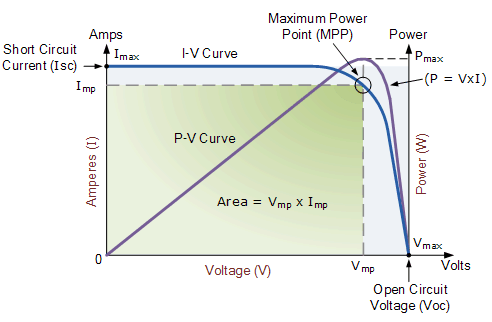
\includegraphics[width=0.76\linewidth]{../Pictures/IVcurve1}
		\caption{I-V and P-V curve of a generic solar panel \cite{IVcurves}.}
		\label{fig:mpp}
	\end{center}
\end{figure}


The PV panel's I-V curve is shown in blue in the Figure \ref{IVcurves}
 for a given PV cell's temperature and solar irradiance. As it is well known, the power generated by a PV cell is the product of current and voltage at each point. Hence, the P-V curve of the solar panel can be obtained and it is displayed in purple. From the P-V curve, the maximum power generated by the solar panel ($P_{max}$) is obtained. This maximum power corresponds to the MPP and takes place for a specific combination of voltage ($V_{mpp}$) and current ($I_{mpp}$). Therefore, the ideal operating point of a PV panel corresponds to the MPP which varies according to the level of solar radiation and the temperature \cite{handbook}. 

There are different types of photovoltaic systems, however, the most common PV systems implemented nowadays are grid-connected \cite{handbook}. This type of PV system is mainly composed of a solar array, a DC-DC converter with an MPPT controller unit and an inverter, as shown in Figure \ref{fig:PVsystemblocks}. 

\begin{figure}[htbp]
	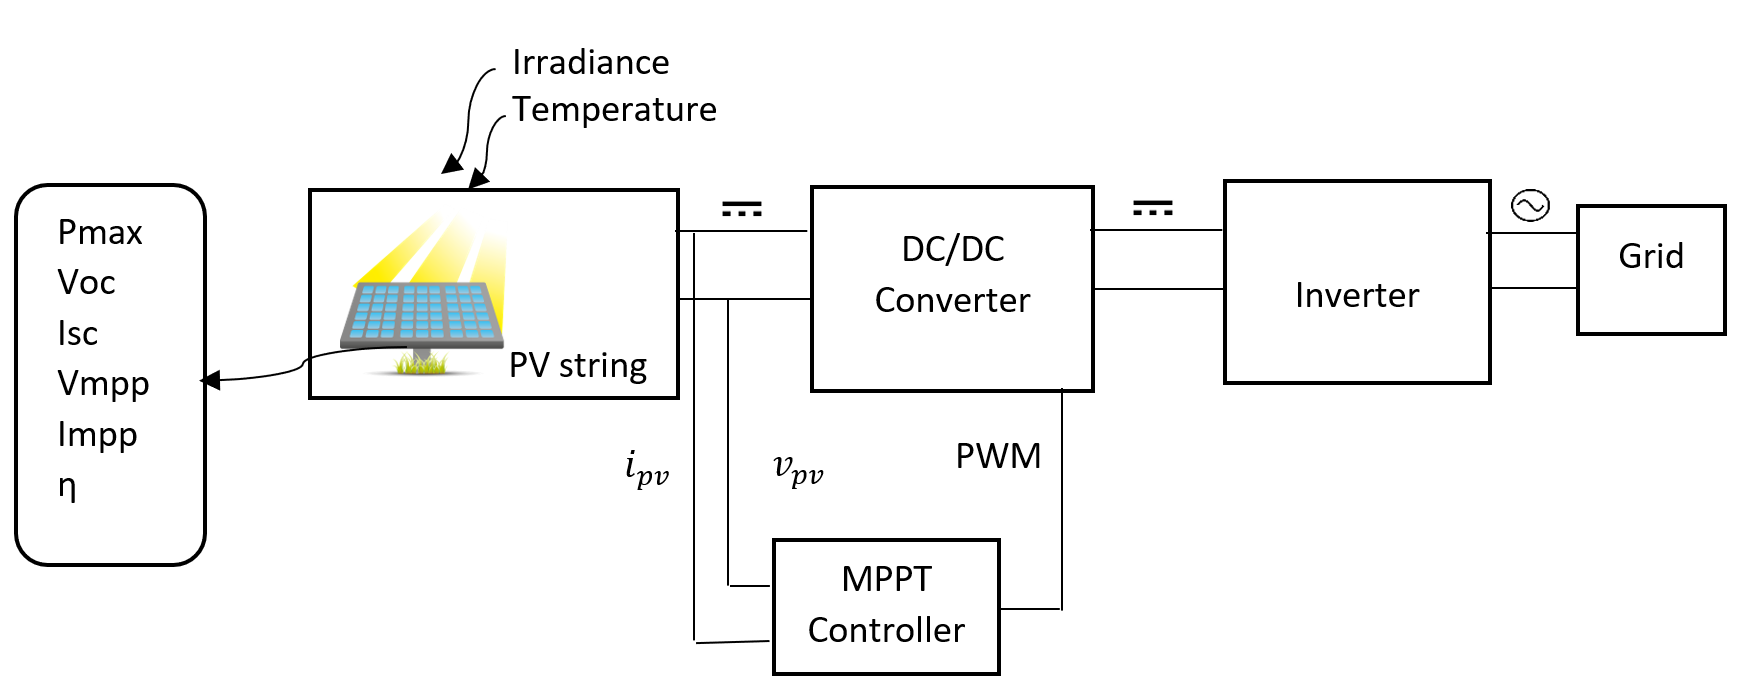
\includegraphics[width=\linewidth]{../Pictures/PV_system_blocks}
	\caption{Basic block diagram of a PV system.}
	\label{fig:PVsystemblocks}
\end{figure}

As mentioned at the begining of the chapter, PV modules can be connected to each other resulting in a PV array/string which generates electrical energy in the form of direct current. The MPPT controller unit takes the PV array's output voltage and current as input variables in order to calculate the corresponding duty cycle for tracking the MPP. The duty cycle is the input of a Pulse Width Modulation (PWM) block \todo{Maybe it is better to explain what the PWM is exactly doing TL. Like this better? Or you think we should explain in detail how the PWM generates the pulses? Stef}. The PWM is used to generate the pulses for the switching components of the DC-DC converter in order to get the PV array to work continuously at its MPP. The output of the DC-DC converter is connected to an inverter to convert the DC electric energy in an AC electrical signal compatible with the grid. 

